\subsection{Grobplanung zuerst}
\label{grob}
	Keine Sorge, deine \textit{Studiengrobplanung} ist ein abstraktes Konzept, du wirst sie nirgends aufschreiben und einreichen müssen, du kannst also große Teile davon so oft ändern wie du möchtest. Aber Vorsicht: Zum einen studiert es sich besser, wenn man von Anfang an weiß, wo es hin geht, zum anderen gibt es gewisse Enscheidungen, die man später nicht mehr ändern kann, wie z.B. das Nebenfach.
	%bla raus! (joke)
	%Aber dazu später mehr\ldots

\subsubsection{Wie viele Credit Points?}
	Standardmäßig sind 30 Credit Points pro Semester vorgesehen - so hat man nach 6 Semestern den Bachelor und nach weiteren 4 den Master in der Tasche. Man ist dann aber auch zeitlich sehr ausgelastet, und für Urlaub, Familie und Nebenjob bleibt nicht unbedingt Zeit. Wenn man im Master außerdem mit Zulassungsauflagen gesegnet ist, sind dies bis zu 15 weitere Credit Points, die man irgendwie auf die ersten beiden Semester aufteilen muss. Deshalb ist es hilfreich sich am Anfang des Studiums zu überlegen, wann man wie viele und ggf. sogar welche Module man belegen will.

	Ein weitere Frage am Anfang des Studiums ist die Finanzierung:
	BAFöG-Höchstförderungsdauer, Langzeitstudiengebühren, sowie das
	Ende von Kindergeld, Kindesunterhalt und Famlienversicherung bei
	der Krankenkasse können problematisch sein. Hiwi-Jobs,
	Studienkredite und Stipendien können helfen, aber vielleicht
	wieder Zeit fressen. 

	Was auch immer du nun denkst, wie viele CP du im kommenden Semester belegen möchte, plane vielleicht ein paar Reserve-Punkte ein, also zusätzliche Fächer, die du belegst. Du kannst dann immernoch im laufenden Semester Vorlesungen abbrechen, wenn es doch nicht so spannend ist wie zuerst gedacht (natürlich keine Pflichtveranstaltungen). Durchfallen ist weder eine Schande noch ein großes Problem, da die Prüfungsordnung dir erlaubt, bis zu drei Fächer, bei denen du im 1. Versuch durchgefallen bist, so abzuwählen als hättest du sie nie belegt. Dennoch sollte man es vielleicht mit den Reservefächern nicht übertreiben.

\subsubsection{Nebenfach und Studienrichtung}
\label{nebenfach}
	Im Bachelor musst du, im Master kannst du ein Nebenfach wählen. Die Nebenfach-Enscheidung (ob und welches) will gut überlegt sein, denn der Wechsel ist nur unter sehr speziellen Bedingungen möglich, wenn man erstmal die erste Prüfung geschrieben hat.
 
	Die Studienrichtung ist  optional, aber im Gegensatz zum Nebenfach geht man damit keinerlei Verpflichtung ein. Am Ende des Studiums wird einfach geschaut, ob man 50 (Bachelor) oder 70 (Master) Credit Points in einem artverwanden Bereich erreicht hat und bekommt dann auf Wunsch ein Sonderprädikat aufs Zeugnis. Aber Vorsicht: manche Studienrichtungen erfordern außerdem noch, das man eine gewisse Untermenge von Seminar, Projektarbeit und Abschlussarbeit, sowie eine Mindestanzahl von Praktika im entsprechenden Bereich absolviert hat. Informiere dich also rechtzeitig! Im schlimmsten Fall kann einem aber nur passieren, dass man sich zwar in einer Richtung spezialisiert hat, darüber aber keinen expliziten Nachweis auf dem Zeugnis erhält.

	Beide Entscheidungen (Nebenfach, Studienrichtung) musst du nicht im ersten Semester treffen, sondern kannst dich auch später (aber am besten nicht zu spät) spezialisieren. Um dir dabei zu helfen, sammelt die Fachgruppe Berichte zu den Nebenfächern unter \url{http://fginfo.cs.tu-bs.de/index.php/studium/erfahrungsberichte-zu-den-nebenfachern/}. 

\subsubsection{Welche Fächer gibt es?}
	Die Liste der Fächer ist groß und ständig im Wandel. Offiziell festgelegt sind sie im Modulhandbuch (MHB). Unter \url{https://vorlesungen.tu-bs.de} findest du mit ein bisschen Suchen eine Übersicht über alle Fächer. Diese Fächer kannst du als Informatikstudent belegen - aber nicht alle werden jedes Semester angeboten.

\subsubsection{Der generelle Stundenplan}
	Unter \url{http://theo.iti.cs.tu-bs.de/STP/stundenplan.php} findest du den aktuellen Plan. Dort sind die meisten Veranstaltungen der Informatikmodule eingetragen, allerdings ohne die Nebenfächer und den Schlüsselqualifikations-Pool. Der Stundenplan enthält sowohl Bachelor- als auch Masterfächer. Also musst du für jedes Fach, was du hier findest, erstmal verifizieren ob du die Punkte überhaupt einbringen kannst. Wie du dir vielleicht schon denken kannst, wird dein persönlicher Stundenplan eine Untermenge dieses Mammut-Plans, erweitert um ein paar Veranstaltungen die hier nicht stehen.

	Wenn etwas darauf hindeutet, dass eine bestimmte Vorlesung im Semester angeboten wird, aber im Stundenplan nicht auftaucht, dann hilft eine Suche auf den Institusseiten, und wenn selbst das nicht hilft, eine Mail an den verantwortlichen Professor. Das gleiche gilt, wenn irgendwas komisch wirkt, z.B. wenn im Stundenplan zu einem Fach 5 Übungstermine und kein Vorlesungstermin stehen.

\subsubsection{Auslandsaufenthalt}
	Über Auslandssemester solltest du dich ebenfalls so früh wie möglich mit dem \emph{International Office} (\url{http://tu-braunschweig.de/international}) in Verbindung setzen.

\subsubsection{Mentoren und Beratungsgespräche}
	Laut Studienordnung bekommst du auch einen Mentor zugewiesen - das ist Professor aus der Informatik, der dich bei Entscheidungen zum Studium im persönlichen Gespräch beraten soll. Gerade wenn du weißt, dass du dich spezialisieren möchtest, oder wenn du zumindest mit dem Gedanken spielst, solltest du einen Mentor haben, der aus der jeweiligen Fachrichtung kommt. Wird dir zu Beginn ein völlig fachfremder Mentor zugewiesen, dann kannst du recht formlos darum bitten, diesen zu wechseln. Gespräche mit dem Mentor sind weder verpflichtend noch planmäßig vorgesehen, sondern liegen in deiner eigenen Verantwortung.

	Außer deinem Mentor gibt es noch weitere Ansprechpartner für verschiedenste Anlässe. Die wichtigsten haben wir für dich unter \url{http://fginfo.cs.tu-bs.de/index.php/kontakt/ansprechpartner/} zusammengefasst.
\begin{center}
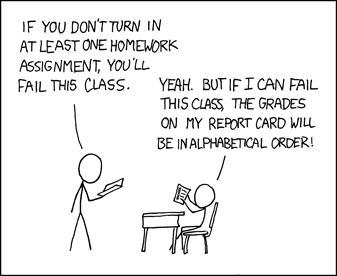
\includegraphics[totalheight=6cm]{bilder/XKCD/priorities}
\end{center}
